%!TEX root = ../dissertation_vkslm.tex

\chapter{Results} \label{ch:results}

As described in Chapter \ref{ch:exp}, two different experiments were
carried out to evaluate the synthetic signatures generated with our proposed method. Namely, we intend to measure how close the synthetic signatures are to real ones and to verify the feasibility of increasing the enrollment dataset with synthetic signatures. The goal of the experiments are:
\begin{itemize}
  \item Measure the quality of the synthetic images;
  \item Assess whether using synthetic signatures effects the recognition performance of an offline signature verification system; and
  \item Analyze the feasibility of using real and synthetic signatures
  on the enrollment set.
\end{itemize}

We compare our results with a state-of-the-art method, particularly the approach proposed by Diaz \textit{et al.} \cite{diaz2014generation}. Specifically, our proposed method is compared with the ``Image enhanced'' synthetic signatures made available as part of the BiosecurID \cite{biosecurid} dataset. The reported EER is achieved for both approaches in the same experimental conditions.

The recognition rates of three types of offline signatures are reported: 
\begin{inlinelist}
  \item real offline signatures, which are the corresponding real offline samples of the online signatures used to generate the synthetic samples, they serve us as a ground-truth, i.e., the ideal synthetic signature should be similar to it;
  \item synthetic signatures generated with the method proposed by Diaz \textit{et al.} \cite{diaz2014generation};
  \item synthetic signatures created with our proposed method
\end{inlinelist}.

\section{Synthetic Signatures in Comparison to Real Signatures - Experiment 1}
In order to evaluate the performance of the synthetic signature signatures described in Chapter \ref{ch:method} and the state-of-the-art, two scenarios were experimented: 
\begin{itemize}
\item Mono-session: signatures from the first session on the enrollment set; and
\item Multi-session: one signature per session.
\end{itemize}


\begin{table}[!htb]
%% increase table row spacing, adjust to taste
\renewcommand{\arraystretch}{1.3}
% if using array.sty, it might be a good idea to tweak the value of
% \extrarowheight as needed to properly center the text within the cells
\caption{EER for real, synthetic samples from Diaz \textit{et al.} \cite{diaz2014generation} and our proposed method synthetic offline signatures, for all the approaches considered under the two possible scenarios (i.e., random and skilled forgeries)}
\label{exp1_results_table}
\centering
%% Some packages, such as MDW tools, offer better commands for making tables
%% than the plain LaTeX2e tabular which is used here.
\begin{tabular}{|l|l|l|l|}
    \hline
    \multicolumn{1}{|c|}{\multirow{2}{*}{\textbf{Mode}}} & \multicolumn{3}{c|}{\textbf{Skilled Forgeries}}          \\ \cline{2-4} 
    \multicolumn{1}{|c|}{}                               & \textbf{Real} & \textbf{Diaz \textit{et al.}} & \textbf{Proposed method} \\ \hline
    \textbf{mono-session}                                & 20.28\%            & 23.19\%            & 18.38\%                       \\ \hline
    \textbf{multi-session}                               & 17.59\%            & 22.27\%            & 16.48\%                       \\ \hline
    \multirow{2}{*}{}                                    & \multicolumn{3}{c|}{\textbf{Random Forgeries}}           \\ \cline{2-4} 
    & \textbf{Real} & \textbf{Diaz \textit{et al.}} & \textbf{Proposed method} \\ \hline
    \textbf{mono-session}                                & 9.07\%            & 10.65\%            & 9.99\%                       \\ \hline
    \textbf{multi-session}                               & 5.60\%            & 10.00\%            & 6.48\%                       \\ \hline
\end{tabular}

\end{table}

Table \ref{exp1_results_table} shows the EER achieved by the
real and the synthetic signatures databases. We observe that under the skilled forgeries scenario our proposed method synthetic signatures EERs yields better performance than both the real dataset and the synthetic signatures generated by Diaz \textit{et al.}. On the random forgeries test, we can identify that, under the random forgeries scenario, the EER results achieved by the real, and both types of synthetic signatures are close to each other. Specifically, under the mono-session scenario, the system's performance for the real signatures was 9.07\%, while the synthetic samples from Diaz \textit{et al.} and our proposed method achieved 10.65\% and 9.99\%, respectively. However, on the multi-session test, the signatures from Diaz \textit{et al.} achieved 10.00\% ERR, while the real signatures and our proposed method EER was 5.60\% and 6.48\%, respectively.


In Figure \ref{exp1} (left - mono-session, right - multi-session) we
may observe that the behavior of the system with real (gray dotted) and our proposed method synthetic signatures are quite similar, regardless of
the training protocol or the scenario considered. Nevertheless, our proposed method synthetic samples achieved a better discriminative power for skilled forgeries.
\begin{figure*}[!htb]
    \centering
    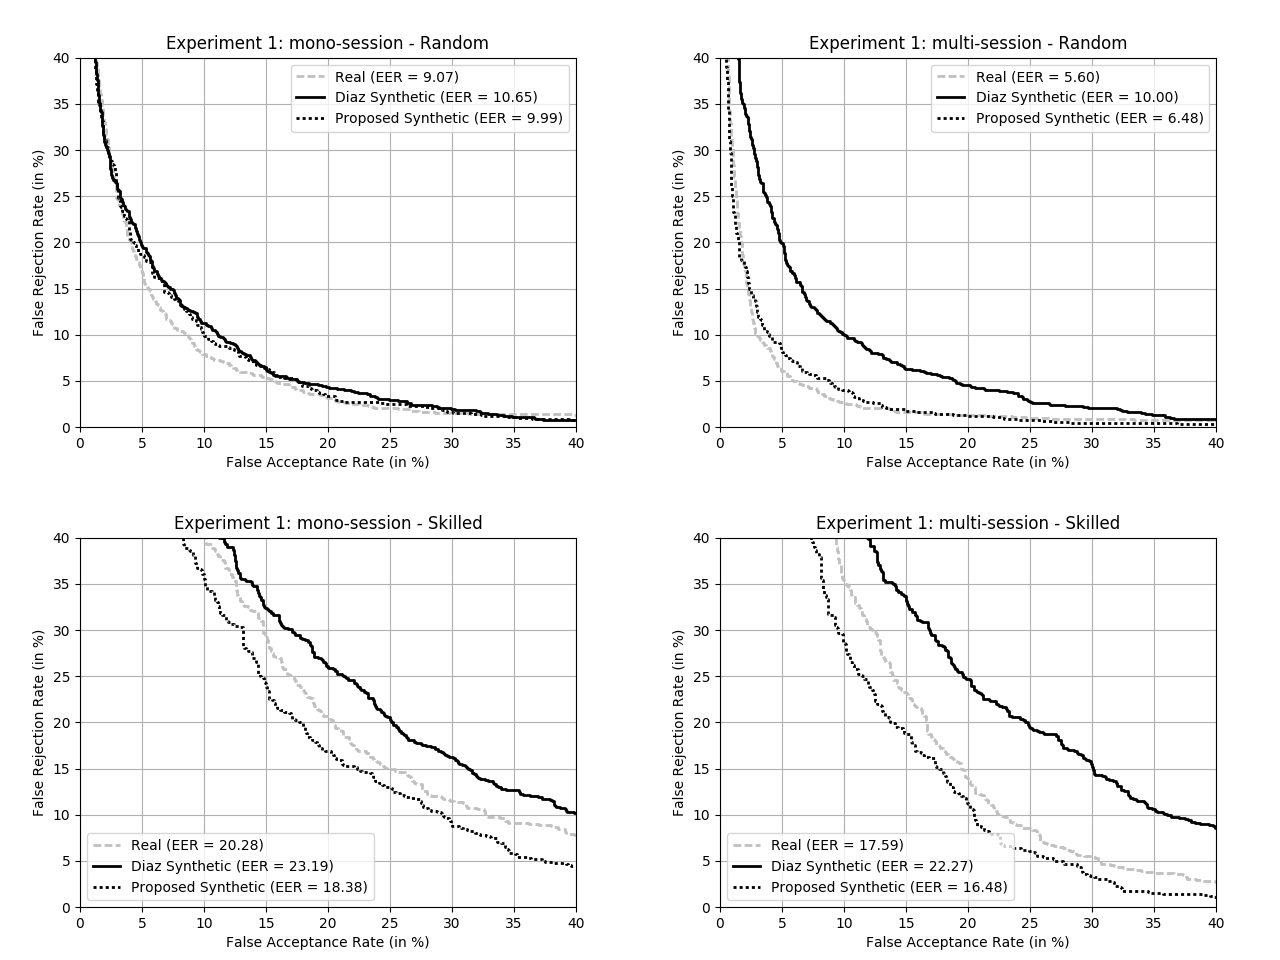
\includegraphics[width=1.05\textwidth]{rocs/experiment1}
    % where an .eps filename suffix will be assumed under latex, 
    % and a .pdf suffix will be assumed for pdflatex; or what has been declared
    % via \DeclareGraphicsExtensions.
    \caption{DET curves for real offline signatures and synthetic signatures (from Diaz \textit{et al.} and our proposed method), for the first experiment (mono-session and multi-session enrollment), for the two scenarios considered (random and skilled impostors)}
    \label{exp1}
\end{figure*}

Moreover, in Figure \ref{fig:box_exp1} we can see that when running the experiments 30 times, the results are consistent, with a low dispersion around the average. We can notice that our proposed method is able to produce synthetic signatures comparable to the real signatures.


\begin{figure*}[!htb]
\centering
 \subfloat[mono-session - random forgeries]{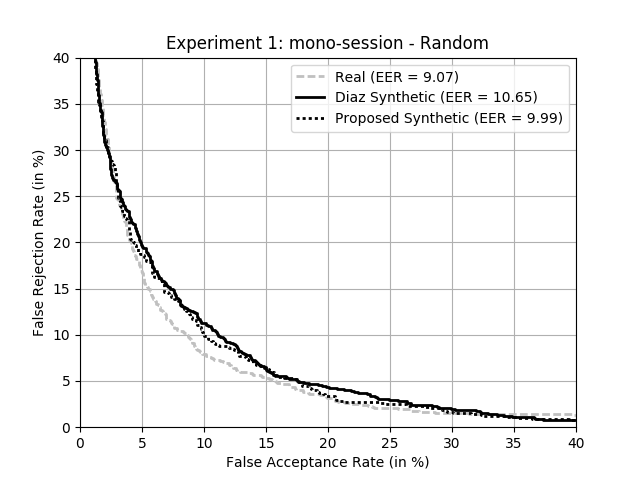
\includegraphics[width=1.3in]{boxplot/mono-random.png}} 
\hspace*{0.2in} % separation between the subfigures
\subfloat[mono-session - skilled forgeries] {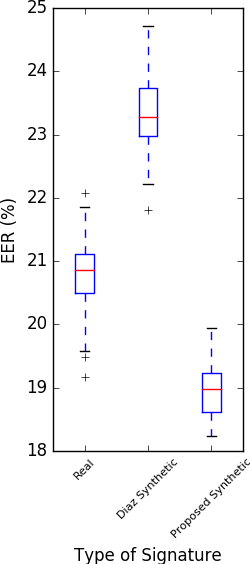
\includegraphics[width=1.3in]{boxplot/mono-skilled.png}}
\hspace*{0.3in} % separation between the subfigures
\subfloat[multi-session - random forgeries]{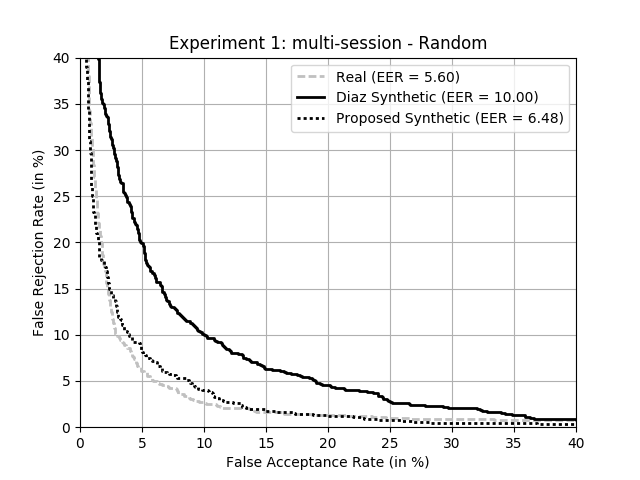
\includegraphics[width=1.3in]{boxplot/multi-random.png}} 
\hspace*{0.2in} % separation between the subfigures
\subfloat[multi-session - skilled forgeries] {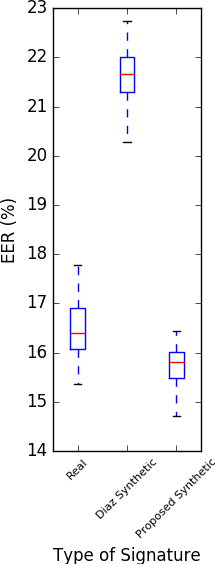
\includegraphics[width=1.3in]{boxplot/multi-skilled.png}}
\caption{Boxplot comparison for running 30 times the Experiment 1 - mono-session scenario and multi-session. (a) mono-session scenario, random forgeries, (b) mono-session scenario, skilled forgeries, (c) multi-session scenario, random forgeries, (d) multi-session scenario, skilled forgeries. } \label{fig:box_exp1}
\end{figure*}

\section{Feasibility of Synthetically Increasing the Enrollment Samples - Experiment 2}
In the last experiment, the feasibility of synthetically
increasing the signature verification enrollment set is analyzed. As it is described in
Chapter \ref{ch:exp}, three different enrollment sets are considered. The DET curves for the mixed enrollment (real + synthetic, gray dashed line) is shown in Figure \ref{fig:exp2} and the summary of the results is presented in Table \ref{exp2_results_table}. We can observe that a better performance compared to the case with only four real
enrolled samples (black line). Specifically, the EER decreases from 10.26\% to 9.74\% on the random forgeries scenario and from 21.55\% to 19.17\% for skilled forgeries, respectively. The addition of synthetic samples for training thus leads to better recognition results.
\begin{figure}[!htb]
    \centering
    

    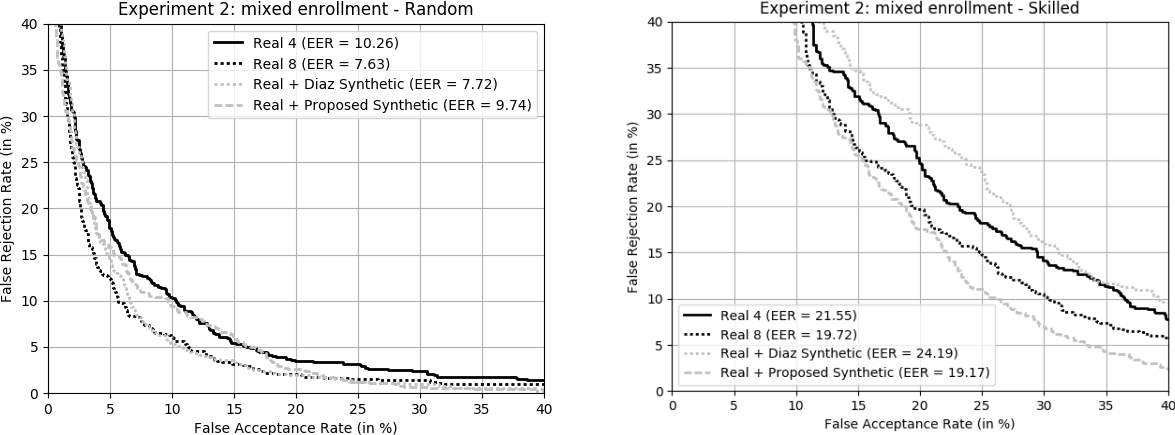
\includegraphics[width=4.5in]{rocs/experiment2}
    % where an .eps filename suffix will be assumed under latex, 
    % and a .pdf suffix will be assumed for pdflatex; or what has been declared
    % via \DeclareGraphicsExtensions.
    \caption{DET curves for real offline signatures and synthetic signatures (from Diaz \textit{et al.} and our proposed method), for the second experiment, for the two scenarios considered (random and skilled impostors)}
    \label{fig:exp2}
\end{figure}

\begin{table}[!htb]
    %% increase table row spacing, adjust to taste
    \renewcommand{\arraystretch}{1.3}
    % if using array.sty, it might be a good idea to tweak the value of
    % \extrarowheight as needed to properly center the text within the cells
    \caption{EER for real, synthetic samples from Diaz \textit{et al.} \cite{diaz2014generation} and our proposed method synthetic offline signatures for the Experiment 2 under the two possible scenarios, i.e., random (RF) and skilled forgeries (SF)}
    \label{exp2_results_table}
    \centering
    %% Some packages, such as MDW tools, offer better commands for making tables
    %% than the plain LaTeX2e tabular which is used here.
    \begin{tabular}{|l|l|l|}
        \hline
        \multicolumn{1}{|c|}{\textbf{Genuine Training}} & \multicolumn{1}{c|}{\textbf{SF}} & \textbf{RF} \\ \hline
        \textbf{4 real samples}                                         & 21.55\%                     & 10.26\%                         \\ \hline
        \textbf{4 real + 4 real samples}                       & 19.72\%                      & 7.63\%                        \\ \hline
        \textbf{4 real + 4 synthetic from Diaz \textit{et al.}}                           & 24.19\%                         & 7.72\%                \\ \hline
        \textbf{4 real + 4 synthetic from the Proposed Method}                           & 19.17\%         & 9.74\%                        \\ \hline
    \end{tabular}

\end{table}

It should also be noted that the behavior of the mixed enrollment is similar to the scenario with eight real enrolled samples (i.e., using eight real samples instead of
four real and four synthetic, black line) for skilled forgeries, and even yields a small improvement on the skilled forgery recognition rates. 

Furthermore, we can see in Figure \ref{fig:boxexp2} that when running the experiments for 30 times, the results of our proposed method has a consistent mean, with
a lower variance around the average. In addition to achieving a comparable EER to using 8 real samples on the enrollment set on the random forgery and skilled forgery scenario.

\begin{figure}[!htb]
\centering
 \subfloat[mixed enrollment - random forgeries]{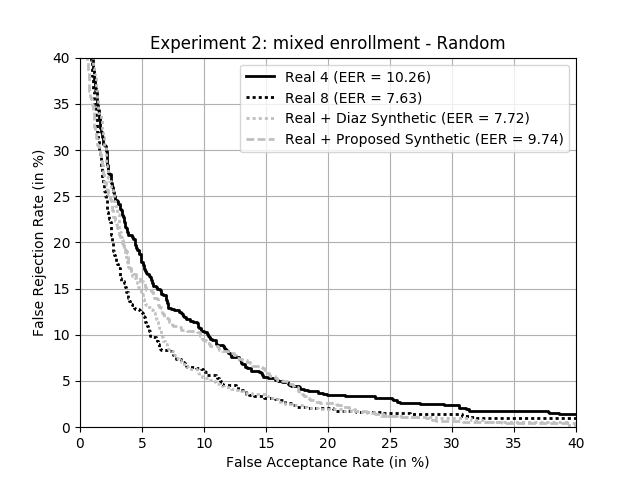
\includegraphics[width=2.0in]{boxplot/mixed-random.png}} 
\hspace*{0.8in} % separation between the subfigures
\subfloat[mixed enrollment - skilled forgeries] {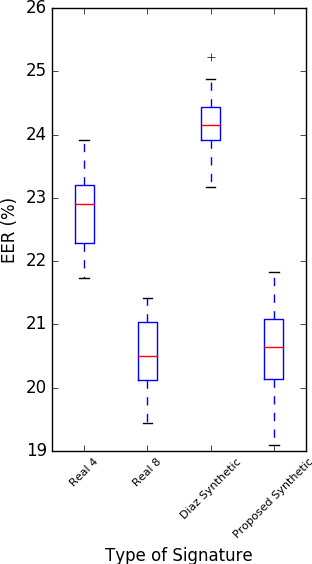
\includegraphics[width=2.0in]{boxplot/mixed-skilled.png}}
\caption{Boxplot comparison for Experiment 2: mixed enrollment - (a) random forgeries and (b) skilled forgeries. } \label{fig:boxexp2}
\end{figure}

It is possible for us to conclude that it is possible to use our proposed system to generate synthetic signatures from dynamic data, when complementary online samples are available, to increase an offline signature dataset, aiming to improve the recognition rate of offline verification systems.




